\documentclass{beamer}
 
\usepackage[utf8]{inputenc}
\usepackage{graphicx}
\graphicspath{{./images/} }
\definecolor{links}{HTML}{2A1B81}
\hypersetup{colorlinks,linkcolor=,urlcolor=links}

\title[] %optional
{Conformal quaternion based mesh (re)construction}
 
\author[] % (optional, for multiple authors)
{Adam Sturge\inst{1}}
 
\institute[] % (optional)
{
  \inst{1}%
  Faculty of Computer Science\\
  University of Toronto
}
 
\date[] % (optional)
{April 5 2017}

\begin{document}
 
\frame{\titlepage}
 
\begin{frame}
\frametitle{About me}
\begin{itemize}
 \item My name is Adam Sturge
 \item I'm a MSc student in the numerical computing group (more statistics honestly)
 \item I majored in Applied mathematics, Physics, and Computer Science at the Memorial University of Newfoundland; my home province.
 \item I worked at EA games for about 3 years doing tools/automation/data analysis
\end{itemize}
\end{frame}

\begin{frame}
\frametitle{What are quaternions?}
\begin{itemize}
 \item Quaternions are a Division Algebra
 \item You can consider them as an extension of the complex numbers with 3 complex coordinates instead of just 1
 \item $\lambda = a + b\boldsymbol{i} + c\boldsymbol{j} + d\boldsymbol{k} = (a,b,c,d)$
 \item Multiplication is not commutative. $ab \neq ba$
 \item $\bar{\lambda} = a - b\boldsymbol{i} - c\boldsymbol{j} - d\boldsymbol{k}$
 \item $||\lambda|| = \sqrt{a^2 + b^2 + c^2 + d^2}$
 \item $\lambda^{-1} = \frac{\bar{\lambda}}{||\lambda||}$ 
 \item $\lambda \in \mathbb{H}$
\end{itemize}
\end{frame}

\begin{frame}
\frametitle{Why are they useful?}
\begin{itemize}
 \item You can embed $\mathbb{R}^{3}$ in $Im\mathbb{H}$. 
 \item Unit quaternions represent a rotation about any axis in $\mathbb{R}^{3}$. If $\vec{u}$ is the axis you want to rotate a vector $\vec{p}$ around by an angle $\theta$ then $\hat{p} = \lambda p \bar{\lambda}$, where $\lambda = (cos(\frac{\theta}{2}),u_{x}sin(\frac{\theta}{2}),u_{y}sin(\frac{\theta}{2}),u_{z}sin(\frac{\theta}{2}))$
 \item Non-unit quaternions represent a rotation and a scale when used in this way
 \item So this operation with quaternions represents a conformal map when applied to the vertices of a triangle
\end{itemize}
\end{frame}

\begin{frame}
\frametitle{Spin Transformations of Discrete Surfaces}
\begin{itemize}
\item \href{https://www.cs.cmu.edu/~kmcrane/Projects/SpinTransformations/}{Spin Transformations of Discrete Surfaces} is a paper where the authors make use of this quaternionic representation of vectors.
\item They build on previous results that show that $2$ surfaces $f$ and $\tilde{f}$ are conformally equivalent if their differentials $df$ and $d\tilde{f}$ are related by 

\begin{equation} \label{continuous_conformal_map}
df = \lambda df \bar{\lambda}
\end{equation}

\item $\lambda$ must apply globally to the whole surface, and as such equation \ref{continuous_conformal_map} may not have a solution
\end{itemize}
\end{frame}

\begin{frame}
\frametitle{Spin Transformations of Discrete Surfaces}
\begin{itemize}
\item The authors introduce a linear integrability condition $(D-\rho)\lambda = 0$ that characterizes all valid quaternions $\lambda$ as presribed changes in \textbf{mean curvature half density} $\rho$ and the dirac operator $D$. 
\item Mean curvature half density: $H|df|$, where H is mean curvature. Is nicer to work with in this contest because a change in mean curvature alone could refer to deformation or just scaling. However a change in $H|df|$ is always indicative of deformation
\end{itemize}
\end{frame}

\begin{frame}
\frametitle{Spin Transformations of Discrete Surfaces}
\begin{figure}[htp]
\centering
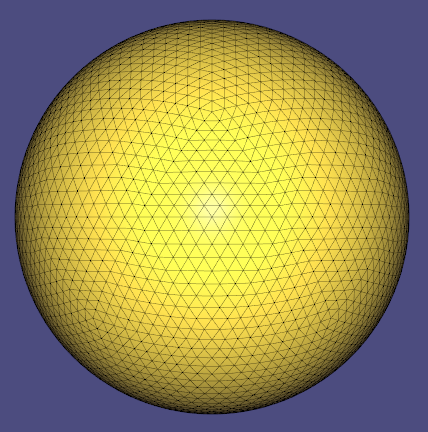
\includegraphics[scale=0.4]{sphere.PNG}\hfill
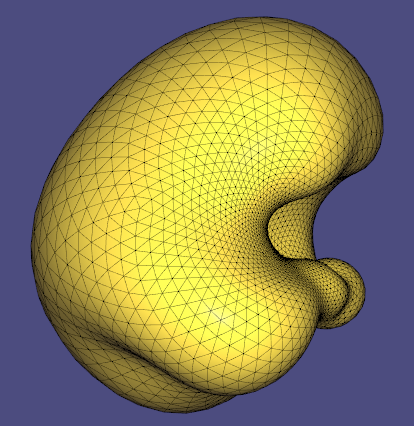
\includegraphics[scale=0.4]{spin_deformed_sphere.PNG}
\caption{sphere deformation}
\label{fig:spin_deformed_sphere}
\end{figure}
\end{frame}

\begin{frame}
\frametitle{My goal}
\begin{itemize}
\item To use their deformation technique to continuously deform a given canonical topological object into a target mesh given a sampling of points from the target mesh
\item It is often easy for human being to tell what topology a mesh should be from looking a point cloud, it's less obvious what geometry it should have.
\end{itemize}
\end{frame}

 
\begin{frame}
\frametitle{Results}
\begin{figure}[htp]
\centering
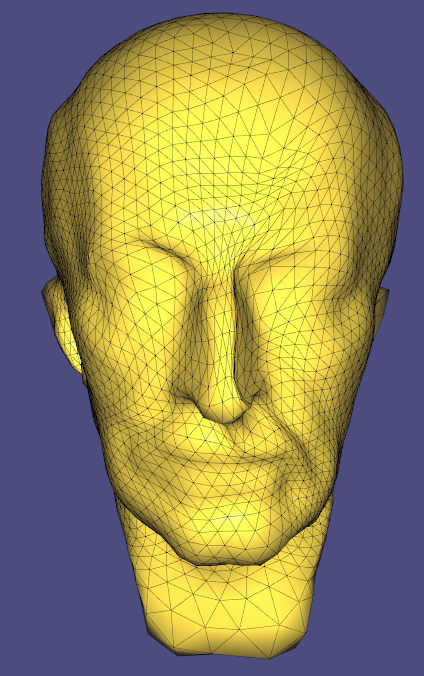
\includegraphics[width=.20\textwidth]{front_sphere_to_head_overnight.PNG}\quad
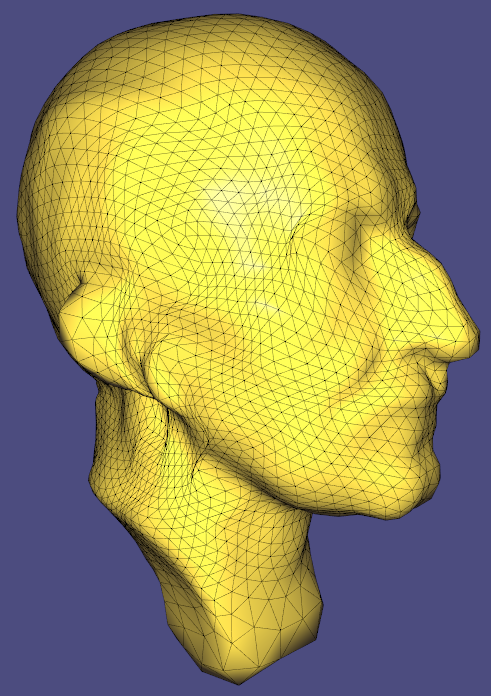
\includegraphics[width=.20\textwidth]{side_sphere_to_head_overnight.PNG}\quad
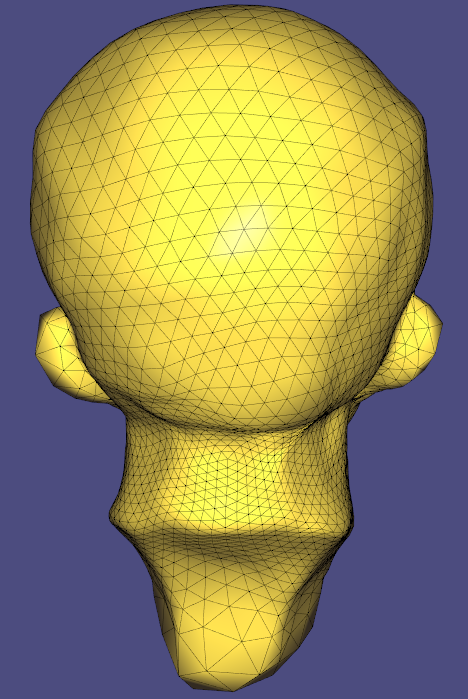
\includegraphics[width=.20\textwidth]{back_sphere_to_head_overnight.PNG}

\medskip

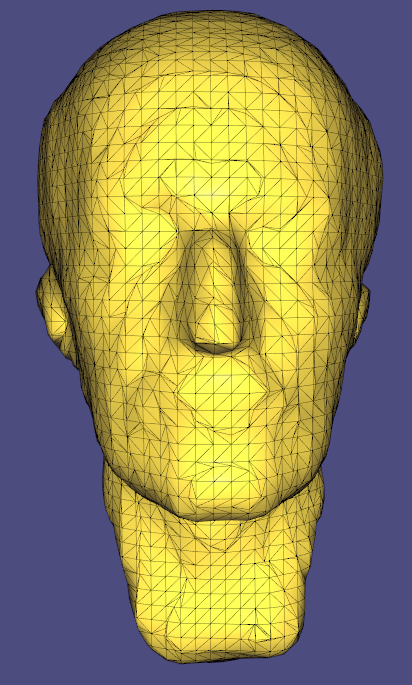
\includegraphics[width=.20\textwidth]{front_poisson.PNG}\quad
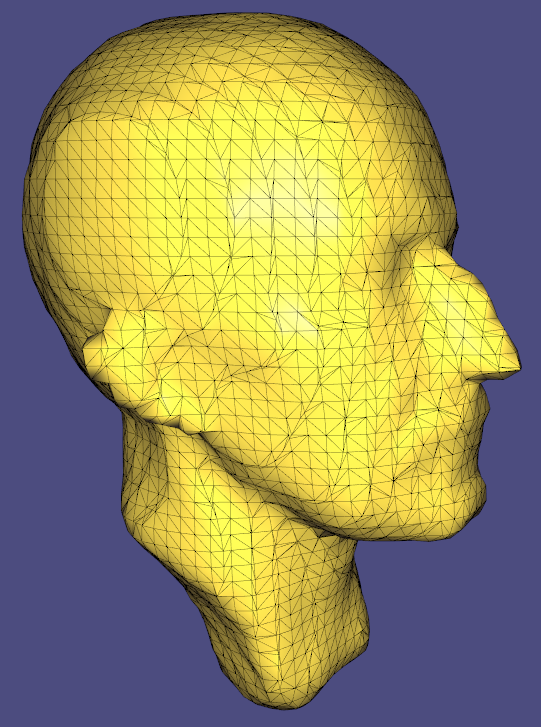
\includegraphics[width=.20\textwidth]{side_poisson.PNG}\quad
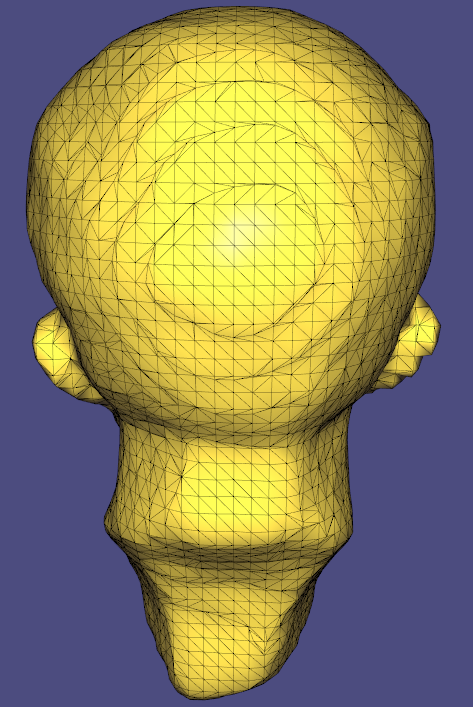
\includegraphics[width=.20\textwidth]{back_poisson.PNG}
\caption{Top : quaternion deformation. Bottom : Poisson reconstruction assignment}
\label{fig:sphere_to_head_final_results}
\end{figure}
\end{frame}


\begin{frame}
\frametitle{Results}
\begin{figure}[htp]
\centering
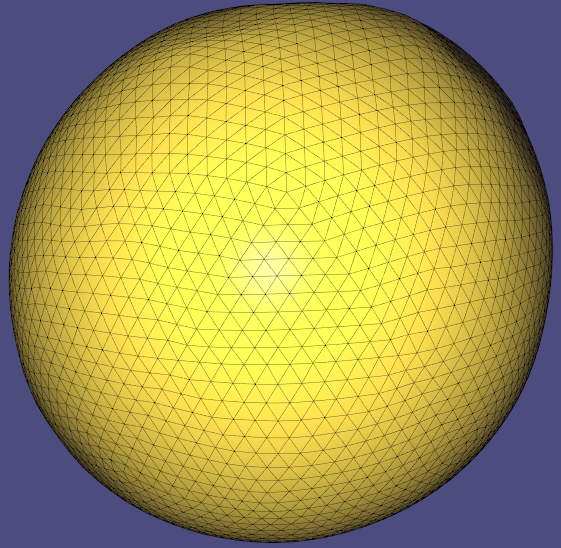
\includegraphics[width=.20\textwidth]{10.PNG}\quad
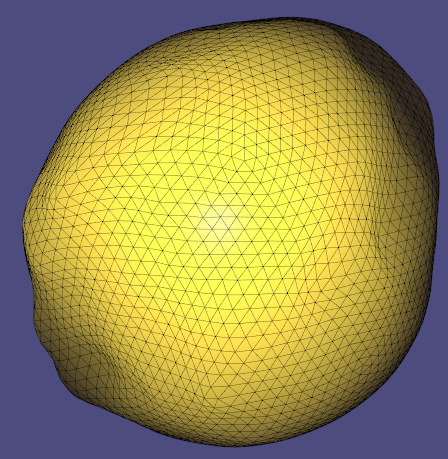
\includegraphics[width=.20\textwidth]{20.PNG}\quad
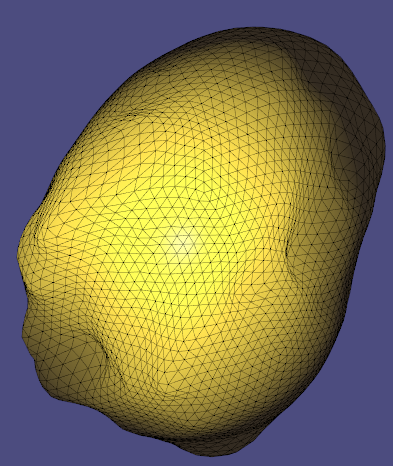
\includegraphics[width=.20\textwidth]{30.PNG}

\medskip

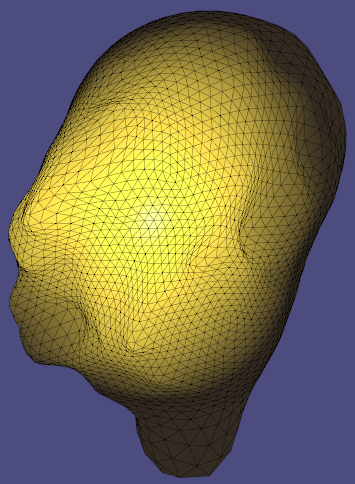
\includegraphics[width=.20\textwidth]{40.PNG}\quad
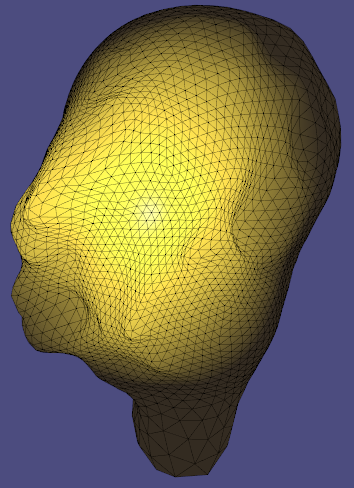
\includegraphics[width=.20\textwidth]{50.PNG}\quad
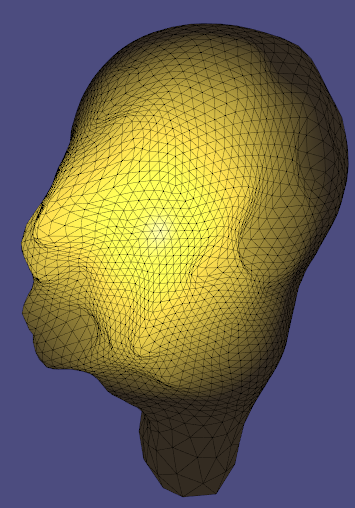
\includegraphics[width=.20\textwidth]{60.PNG}
\caption{gradient decent iterations (with resampling): 10, 20, 30, 40, 50, 60}
\label{fig:iterations}
\end{figure}
\end{frame}


\begin{frame}
\frametitle{Results}
\href{https://drive.google.com/open?id=0Bxe_aqElJ61ULXk0S284Y25xME0}{DEMO}
\end{frame}

\begin{frame}
\frametitle{Mesh fitting procedure}
\begin{itemize}
\item I decided to go with an Iterative Closest Point (ICP) algorithm to deform the meshes. There are two approaches
\item First sample the \textbf{seed mesh} and for each sample find the closest point in the \textbf{target point cloud}
\item First sample the \textbf{target point cloud} and project the samples onto \textbf{seed mesh}
\item After collecting the samples, use them to minimize some energy
\end{itemize}
\end{frame}

\begin{frame}
\frametitle{Minimization energy}
\begin{itemize}
\item Energy to minimize (point to point)
\begin{equation}
E(\lambda) = \int_{\Omega}||X(\lambda) - P||^{2}d\Omega \approx \sum_{i=0}^{k}||x_{i}(\lambda) - p_{i}||^{2}
\end{equation}
\item Energy to minimize (point to plane)
\begin{equation}
E(\lambda) = \sum_{i=0}^{k}((x_{i}(\lambda) - p_{i}) \cdot n_{i})^{2}
\end{equation}
\end{itemize}
\end{frame}

\begin{frame}
\frametitle{Discretization}
\begin{itemize}
\item How to discretize this problem for triangle meshes?
\item Assign each vertex $v_{i}$ a quaternion $\lambda_{i}$
\item Solve least squares problem for new vertex positions $\tilde{v_{i}}$
\item Instead focus on finding a quaternion vector $\vec{\lambda} = (\lambda_{0},\lambda_{1}, \ldots, \lambda_{n} )$ to deform vertices
\item More details in \href{https://www.cs.cmu.edu/~kmcrane/Projects/SpinTransformations/}{Spin Transformations of Discrete Surfaces} Keenan et al
\end{itemize}
\end{frame}

\begin{frame}
\frametitle{How to minimize?}
\begin{itemize}
\item The relationship between $\vec{\lambda}$ and $x_{i}(\vec{\lambda})$ is pretty complicated. 
\item $E(\vec{\lambda})$ is a functional, so we can use gradient decent
\item $\vec{\lambda} \rightarrow \vec{\lambda} + \alpha\frac{\nabla E(\vec{\lambda})}{||\nabla E(\vec{\lambda})||}$
\item Use reverse mode autodifferentiation to algorithmically compute gradient
\item Start from identity transform where each $\lambda_{i} = (1,0,0,0)$
\item Do not need the linear integrability condition from Keenan et al since we are taking a guess and refining it
\end{itemize}
\end{frame}

\begin{frame}
\frametitle{Issues}
\begin{itemize}
\item Each iteration of gradient decent involves solving a large least squares problem, which can take up to 1 sec to solve
\item Sampling can take a long time
\item Storing the large matricies involved requires a lot of RAM, peaking around 20GB on my home PC. This could probably be mitigated somewhat be optimized code
\item Gradient decent is prone to getting stuck in local optima (lack of fine detail)
\item Introduces cloth like ripples onto the resulting surface
\end{itemize}
\end{frame}

\begin{frame}
\frametitle{Future work}
\begin{itemize}
\item Look into spatial data structures to speed up sampling
\item Find a closed form solution for the gradient so I don't need autodifferentiion
\item Find closed form equation for optimal $\vec{\lambda}$ instead of using gradient decent
\end{itemize}
\end{frame}

\end{document}